\clearpage

\subsection{Opaque without Survivability}\label{ILP_Opaque_Survivability}
\begin{tcolorbox}	
\begin{tabular}{p{2.75cm} p{0.2cm} p{10.5cm}} 	
\textbf{Student Name}  &:& Tiago Esteves    (October 03, 2017 - )\\
\textbf{Goal}          &:& Implement the ILP model for the opaque transport mode without survivability.
\end{tabular}
\end{tcolorbox}

\subsubsection{Model description}

First, for a better understanding of the functions and variables used in the ILP, a table \ref{description_opaque} will be created with all indexes, inputs and variables and with their respective description.\\

\begin{table}[h!]
\centering
\begin{tabular}{ |p{1cm}||p{13cm}|}
 \hline
 \multicolumn{2}{|c|}{Description of notation used in the objective function} \\
 \hline
 \hline
 $i$ & index for start node of a physical link \\
 $j$ & index for end node of a physical link \\
 $o$ & index for node that is origin of a demand \\
 $d$ & index for node that is destination of a demand \\
 $c$ & index for bit rate of the client signal \\
 $($ i,j $)$ & physical link between the nodes $i$ and $j$ \\
 $($ o,d $)$ & demand between the nodes $o$ and $d$ \\
 $C$ & set of the client signal \\
 $f_{ij}^{od}$ & binary variable indicating if link between the nodes $i$ and $j$ is used in the path between nodes $o$ and $d$ \\
 $L_{ij}$ & binary variable indicating if link between the nodes $i$ and $j$ is used \\
 $W_{ij}$ & number of optical channels between the nodes $i$ and $j$\\
 $B_c $ & client signals granularities $($1.25, 2.5, 10, 40, 100$)$ \\
 $D_{odc}$ & client demands with bit rate $c$ between nodes $o$ and $d$ \\
 $G_{ij}$ & network topology in form of adjacency matrix \\
 \hline
\end{tabular}
\caption{Table with description of variables}
\label{description_opaque}
\end{table}

Before carrying out the description of the objective function we must take into account the following particularity of this mode of transport:
\begin{itemize}
  \item $N_{OXC,n}$ = 0, \quad $\forall$ n
  \item $N_{EXC,n}$ = 1, \quad $\forall$ n that process traffic
\end{itemize}

\vspace{11pt}
The objective function of following the ILP is a minimization of the CAPEX through the equation \ref{Capex} where in this case for the cost of nodes we only have in consideration the electric cost \ref{Capex_Node_EXC} because of the particularity previously mentioned.
In this case the value of $P_{exc,c,n}$ is obtained by equation \ref{EXC_pexc1_opaque} for long-reach and by the equation \ref{EXC_pexc2_opaque} for short-reach.\\

\newpage
As previously mentioned, equation \ref{EXC_pexc1_opaque} refers to the number of long-reach ports of the electrical switch with bit-rate -1 in node n, $P_{exc,-1,n}$, i.e. the number of line ports of node n which can be calculated as

\begin{equation}
P_{exc,-1,n} = \sum_{j=1}^{N} w_{nj}
\label{EXC_pexc1_opaque}
\end{equation}

\vspace{11pt}
where $w_{nj}$ is the number of optical channels between node $n$ and node $j$.

\vspace{11pt}
As previously mentioned, equation \ref{EXC_pexc2_opaque} refers to the number of sort-reach ports of the electrical switch with bit-rate c in node n, $P_{exc,c,n}$, i.e. the number of tributary ports with bit-rate c in node n which can be calculated as

\begin{equation}
P_{exc,c,n} = \sum_{d=1}^{N} D_{nd,c}
\label{EXC_pexc2_opaque}
\end{equation}

\vspace{11pt}
where $D_{nd,c}$ are the client demands between nodes $n$ and $d$ with bit rate $c$.

\vspace{11pt}
In this case there is the following particularity:

\begin{itemize}
  \item When $n$=$d$ the value of client demands is always zero, i.e, $D_{nn,c}=0$
\end{itemize}


\vspace{17pt}
The objective function, to be minimized, is the expression \ref{ILPOpaque_CAPEX}.\\

$subject$ $to$
\begin{equation}
\sum_{j\textbackslash \{o\}} f_{ij}^{od} = 1  \qquad \qquad \qquad \qquad \qquad \qquad \qquad \qquad \qquad \qquad
\forall(o,d) : o < d, \forall i: i = o
\label{ILPOpaque1_Surv}
\end{equation}

This constraint are equal to the constraint \ref{ILPOpaque1_CAPEX} assuming that Z variable has the value of 1.

\begin{equation}
\sum_{j\textbackslash \{o\}} f_{ij}^{od} = \sum_{j\textbackslash \{d\}} f_{ji}^{od}   \qquad \qquad \qquad \qquad \qquad \qquad \qquad \qquad
\forall(o,d) : o < d, \forall i: i \neq o,d
\label{ILPOpaque2_Surv}
\end{equation}

This constraint are equal to the constraint \ref{ILPOpaque2_CAPEX}.

\begin{equation}
\sum_{j\textbackslash \{d\}} f_{ji}^{od} = 1  \qquad \qquad \qquad \qquad \qquad \qquad \qquad \qquad \qquad \qquad
\forall(o,d) : o < d, \forall i: i = d
\label{ILPOpaque3_Surv}
\end{equation}

This constraint are equal to the constraint \ref{ILPOpaque3_CAPEX} assuming that Z variable has the value of 1.
\newpage
\begin{equation}
\sum_{o=1} \sum_{d=o+1} \left(f_{ij}^{od} + f_{ji}^{od}\right) \sum_{c\in C} (B\left(c\right) D_{odc}\leq \tau W_{ij} G_{ij} \qquad \qquad \qquad
\forall(i,j) : i < j
\label{ILPOpaque4_Surv}
\end{equation}

This restriction is considered grooming constraint, so it means the total client traffic flows can not be greater than the capacity of optical transmission system on all links where $\tau$ is always 100.

\begin{equation}
W_{ij} \leq K_{ij} L_{ij} \qquad  \qquad \qquad \qquad \qquad \qquad \qquad \qquad \qquad \qquad \qquad \qquad \forall(i,j) : i < j
\label{ILPOpaque5_Surv}
\end{equation}

This restriction concerns the capacity of the optical channels which must be less or equal to the maximum number of optical channels. For any situation the maximum number of optical channels supported by each transmission system is 100, i.e., $K_{ij}$ = 100.

\begin{equation}
f_{ij}^{od} , f_{ji}^{od} \in \{0,1\}   \qquad \qquad \qquad \qquad \qquad \qquad \qquad \qquad \qquad
\forall(i,j) : i < j, \forall(o,d) : o < d
\label{ILPOpaque6_Surv}
\end{equation}

The number of flows per demand in this case can be zero if there are no traffic demands or one if considering traffic.

\begin{equation}
W_{ij} \in \mathbb{N}  \qquad \qquad \qquad \qquad \qquad \qquad \qquad \qquad \qquad \qquad \qquad \qquad \qquad
\forall(i,j) : i < j
\label{ILPOpaque7_Surv}
\end{equation}

The last constraint is just needed to ensure the number optical of channels is a positive integer values greater than zero.


\subsubsection{Result description}

To perform the calculations using the implementation of the models described previously it is necessary to use a mathematical software tool. For this we will use MATLAB which is ideal for dealing with linear programming problems and can call the LPsolve through an external interface.
We already have all the necessary to obtain the CAPEX value for the reference network \ref{Reference_Network_Topology}. As described in the subsection of network traffic \ref{Reference_Network_Traffic}, we have three values of network traffic (low, medium and high traffic) so we have to obtain three different CAPEX.
The value of the CAPEX of the network will be calculated based on the costs of the equipment present in the table \ref{table_cost_ilp}.\\


\textbf{Low Traffic Scenario:}\\

In this scenario we have to take into account the traffic calculated in \ref{low_traffic_scenario}. In a first phase we will show the various exiting topologies of the network. The first are the allowed topologies, physical and optical topology, the second are the logical topology for all ODUs and finally the resulting physical and optical topology.\\

\begin{figure}[h!]
\centering
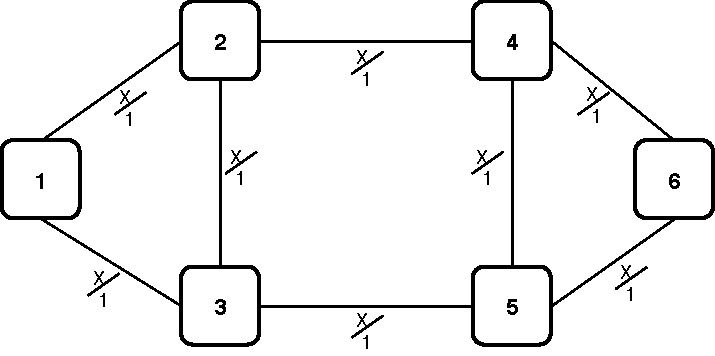
\includegraphics[width=12cm]{sdf/ilp/opaque_survivability/figures/allowed_physical_topology}
\caption{Allowed Physical Topology.}
\label{allowed_physical_low}
\end{figure}

\begin{figure}[h!]
\centering
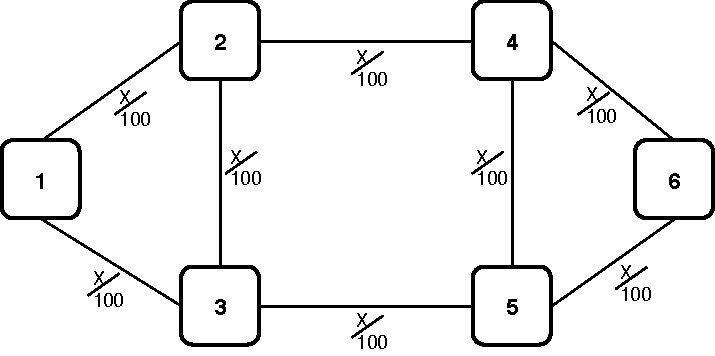
\includegraphics[width=12cm]{sdf/ilp/opaque_survivability/figures/allowed_optical_topology}
\caption{Allowed Optical Topology.}
\label{allowed_optical_low}
\end{figure}

\begin{figure}[h!]
\centering
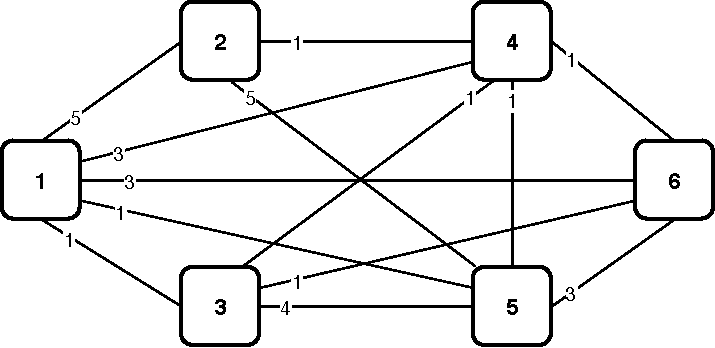
\includegraphics[width=12cm]{sdf/ilp/opaque_survivability/figures/logical_topology_ODU0_low}
\caption{Logical Topology of ODU0.}
\label{logical_ODU0_low}
\end{figure}

\begin{figure}[h!]
\centering
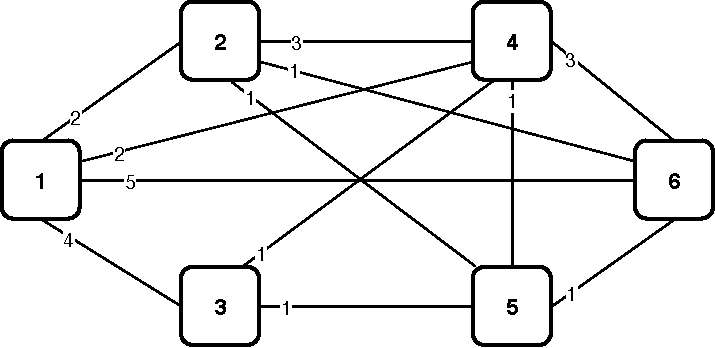
\includegraphics[width=12cm]{sdf/ilp/opaque_survivability/figures/logical_topology_ODU1_low}
\caption{Logical Topology of ODU1.}
\label{logical_ODU1_low}
\end{figure}

\begin{figure}[h!]
\centering
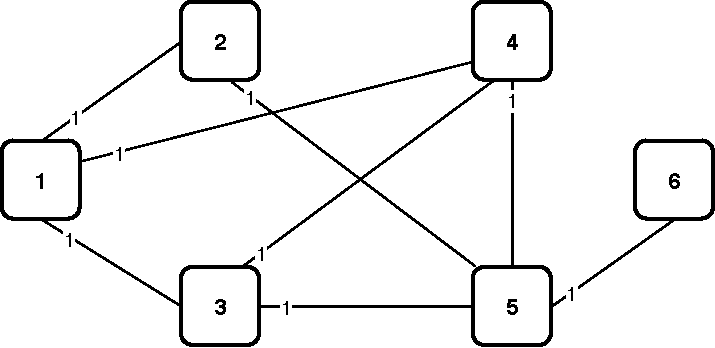
\includegraphics[width=12cm]{sdf/ilp/opaque_survivability/figures/logical_topology_ODU2_low}
\caption{Logical Topology of ODU2.}
\label{logical_ODU2_low}
\end{figure}

\begin{figure}[h!]
\centering
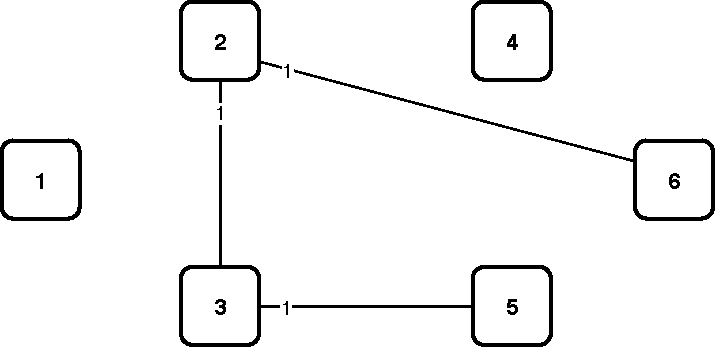
\includegraphics[width=12cm]{sdf/ilp/opaque_survivability/figures/logical_topology_ODU3_low}
\caption{Logical Topology of ODU3.}
\label{logical_ODU3_low}
\end{figure}

\begin{figure}[h!]
\centering
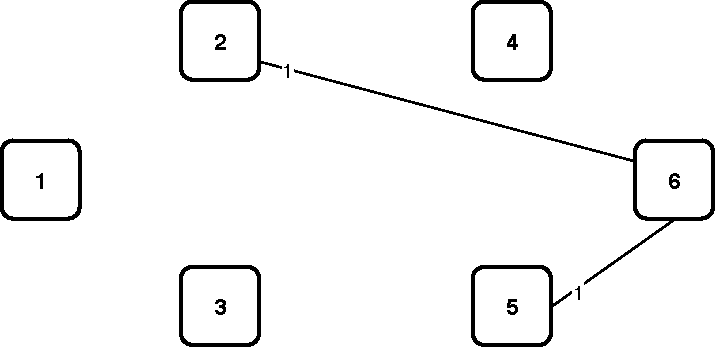
\includegraphics[width=12cm]{sdf/ilp/opaque_survivability/figures/logical_topology_ODU4_low}
\caption{Logical Topology of ODU4.}
\label{logical_ODU4_low}
\end{figure}

\begin{figure}[h!]
\centering
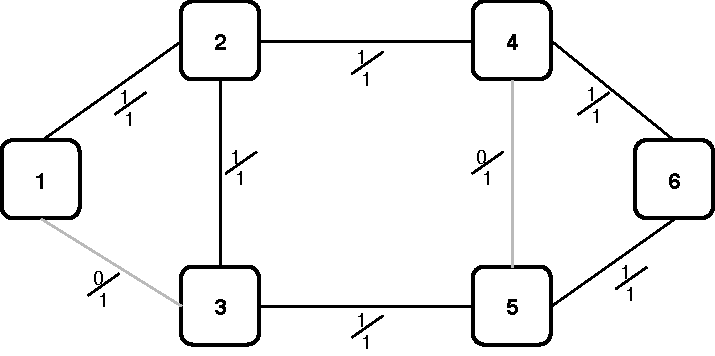
\includegraphics[width=12cm]{sdf/ilp/opaque_survivability/figures/physical_topology_low}
\caption{Physical Topology.}
\label{physical_low}
\end{figure}

\begin{figure}[h!]
\centering
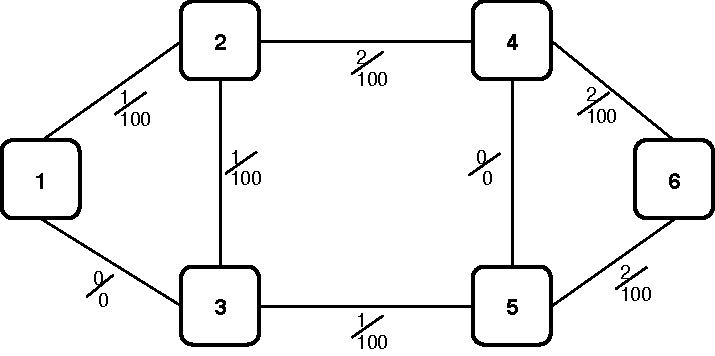
\includegraphics[width=12cm]{sdf/ilp/opaque_survivability/figures/optical_topology_low}
\caption{Optical Topology.}
\label{optical_low}
\end{figure}

In table \ref{link_opaque_surv_ref_low} we can see the number of optical channels and the number of amplifiers for each link calculated through MatLab.\\

\begin{table}[h!]
\centering
\begin{tabular}{|| c | c | c ||}
 \hline
 \multicolumn{3}{|| c ||}{Information regarding links} \\
 \hline
 \hline
 Bidirectional Link & Optical Channels & Amplifiers\\
 \hline
 Node 1 <-> Node 2 & 1 & 4 \\
 Node 1 <-> Node 3 & 0 & 6 \\
 Node 2 <-> Node 3 & 1 & 0 \\
 Node 2 <-> Node 4 & 2 & 6 \\
 Node 3 <-> Node 5 & 1 & 8 \\
 Node 4 <-> Node 5 & 0 & 1 \\
 Node 4 <-> Node 6 & 2 & 7 \\
 Node 5 <-> Node 6 & 2 & 3 \\
 \hline
\end{tabular}
\caption{Table with information regarding links}
\label{link_opaque_surv_ref_low}
\end{table}

\vspace{13pt}
In table \ref{node_opaque_surv_ref_low} we can see the number of connections that each node has, the number of line ports and the number of tributary ports for each node.\\


\begin{table}[h!]
\centering
\begin{tabular}{|| c | c | c | c ||}
 \hline
 \multicolumn{4}{|| c ||}{Information regarding nodes} \\
 \hline
 \hline
 Node & Resulting Nodal Degree & Line Ports & Tributary Ports\\
 \hline
 1 & 1 & 1 & 29 \\
 2 & 3 & 4 & 23 \\
 3 & 2 & 2 & 18 \\
 4 & 2 & 4 & 20 \\
 5 & 2 & 3 & 24 \\
 6 & 2 & 4 & 22 \\
\hline
\end{tabular}
\caption{Table with information regarding nodes}
\label{node_opaque_surv_ref_low}
\end{table}

\vspace{13pt}
Through the information obtained previously on the nodes we can now create tables with detailed information about each node.\\
In each table mentioned below we can see how many ports are connected to a given node and its bit rate (in relation to the line ports) and how many ports are assigned to each different bit rate (in relation to the tributary ports).\\

\newpage
\begin{table}[h!]
\centering
\begin{tabular}{|| c | c | c ||}
 \hline
 \multicolumn{3}{|| c ||}{Detailed description of Node 1} \\
 \hline
 \hline
 1 line ports & 1 connect to Node 2 & 100 Gbits/s \\ \hline
\multirow{3}{*}{29 tributary ports} & 13 & ODU0 \\
 & 13 & ODU1 \\
 & 3 & ODU2 \\
\hline
\end{tabular}
\caption{Table with detailed description of node 1}
\end{table}

\vspace{13pt}
\begin{table}[h!]
\centering
\begin{tabular}{|| c | c | c ||}
 \hline
 \multicolumn{3}{|| c ||}{Detailed description of Node 2} \\
 \hline
 \hline
 \multirow{3}{*}{4 line ports} & 1 connect to Node 1 & \multirow{3}{*}{100 Gbits/s} \\
 & 1 connect to Node 3 & \\
 & 2 connect to Node 4 & \\ \hline
\multirow{5}{*}{23 tributary ports} & 11 & ODU0 \\
 & 7 & ODU1 \\
 & 2 & ODU2 \\
 & 2 & ODU3 \\
 & 1 & ODU4 \\
\hline
\end{tabular}
\caption{Table with detailed description of node 2}
\end{table}

\vspace{13pt}
\begin{table}[h!]
\centering
\begin{tabular}{|| c | c | c ||}
 \hline
 \multicolumn{3}{|| c ||}{Detailed description of Node 3} \\
 \hline
 \hline
 \multirow{2}{*}{2 line ports} & 1 connect to Node 2 & \multirow{2}{*}{100 Gbits/s}\\
 & 1 connect to Node 5 & \\ \hline
\multirow{4}{*}{18 tributary ports} & 7 & ODU0 \\
 & 6 & ODU1\\
 & 3 & ODU2\\
 & 2 & ODU3\\
\hline
\end{tabular}
\caption{Table with detailed description of node 3}
\end{table}

\vspace{13pt}
\begin{table}[h!]
\centering
\begin{tabular}{|| c | c | c ||}
 \hline
 \multicolumn{3}{|| c ||}{Detailed description of Node 4} \\
 \hline
 \hline
 \multirow{2}{*}{4 line ports} & 2 connect to Node 2 & \multirow{2}{*}{100 Gbits/s}\\
 & 2 connect to Node 6 & \\ \hline
\multirow{3}{*}{20 tributary ports} & 7 & ODU0 \\
 & 10 & ODU1 \\
 & 3 & ODU2 \\
\hline
\end{tabular}
\caption{Table with detailed description of node 4}
\end{table}

\newpage
\begin{table}[h!]
\centering
\begin{tabular}{|| c | c | c ||}
 \hline
 \multicolumn{3}{|| c ||}{Detailed description of Node 5} \\
 \hline
 \hline
 \multirow{2}{*}{3 line ports} & 1 connect to Node 3 & \multirow{2}{*}{100 Gbits/s}\\
 & 2 connect to Node 6 & \\ \hline
\multirow{5}{*}{24 tributary ports} & 14 & ODU0 \\
 & 4 & ODU1 \\
 & 4 & ODU2 \\
 & 1 & ODU3 \\
 & 1 & ODU4 \\
\hline
\end{tabular}
\caption{Table with detailed description of node 5}
\end{table}


\begin{table}[h!]
\centering
\begin{tabular}{|| c | c | c ||}
 \hline
 \multicolumn{3}{|| c ||}{Detailed description of Node 6} \\
 \hline
 \hline
 \multirow{2}{*}{4 line ports} & 2 connect to Node 4 & \multirow{2}{*}{100 Gbits/s}\\
 & 2 connect to Node 5 & \\ \hline
\multirow{5}{*}{22 tributary ports} & 8 & ODU0 \\
 & 10 & ODU1 \\
 & 1 & ODU2 \\
 & 1 & ODU3 \\
 & 2 & ODU4 \\
\hline
\end{tabular}
\caption{Table with detailed description of node 6}
\end{table}

\vspace{13pt}
Now through the table \ref{scriptopaque_surv_ref_low} we can see the result of CAPEX obtained with this ILP model.

\begin{table}[h!]
\centering
\begin{tabular}{|| c | c | c | c | c | c | c ||}
 \hline
 \multicolumn{7}{|| c ||}{CAPEX of the Network} \\
 \hline
 \hline
 \multicolumn{3}{|| c |}{ } & Quantity & Unit Price & Cost & Total \\
 \hline
 \multirow{3}{*}{Link Cost} & \multicolumn{2}{ c |}{OLTs} & 12 & 15 000 \euro & 180 000 \euro & \multirow{3}{*}{9 404 000 \euro} \\ \cline{2-6}
 & \multicolumn{2}{ c |}{100 Gb/s Transceivers} & 18 & 5 000 \euro/Gb/s & 9 000 000 \euro & \\ \cline{2-6}
 & \multicolumn{2}{ c |}{Amplifiers} & 56 & 4 000 \euro & 224 000 \euro & \\
 \hline
 \multirow{9}{*}{Node Cost} & \multirow{7}{*}{Electrical} & EXCs & 6 & 10 000 \euro & 60 000 \euro & \multirow{9}{*}{1 862 590 \euro} \\ \cline{3-6}
 & & ODU0 Ports & 60 & 8 \euro/Gb/s & 600 \euro & \\ \cline{3-6}
 & & ODU1 Ports & 50 & 6 \euro/Gb/s & 750 \euro & \\ \cline{3-6}
 & & ODU2 Ports & 16 & 3 \euro/Gb/s & 480 \euro & \\ \cline{3-6}
 & & ODU3 Ports & 6 & 1.5 \euro/Gb/s & 360 \euro & \\ \cline{3-6}
 & & ODU4 Ports & 4 & 1 \euro/Gb/s & 400 \euro & \\ \cline{3-6}
 & & Line Ports & 18 & 1 000 \euro/Gb/s & 1 800 000 \euro & \\ \cline{2-6}
 & \multirow{2}{*}{Optical} & OXCs & 0 & 20 000 \euro & 0 \euro & \\ \cline{3-6}
 & & Ports & 0 & 2 500 \euro/porto & 0 \euro & \\
 \hline
 \multicolumn{6}{|| c |}{Total Network Cost} & 11 266 590 \euro \\
\hline
\end{tabular}
\caption{Table with detailed description of CAPEX}
\label{scriptopaque_surv_ref_low}
\end{table}


Through the formulas mentioned below we can see how all the values of the quantity column were calculated.

\begin{table}[h!]
\centering
\begin{tabular}{|| c | c ||}
 \hline
 OLTs: & \(\displaystyle 2 \sum_{i=1}^{N}\sum_{j=i+1}^{N} L_{ij} \) \\ \hline
 Transceivers: & \(\displaystyle 2 \sum_{i=1}^{N}\sum_{j=i+1}^{N} W_{ij} \) \\ \hline
 Amplifiers: & \(\displaystyle \sum_{i=1}^{N}\sum_{j=i+1}^{N} N^R_{ij} L_{ij} \) \\ \hline
 EXCs: & \(\displaystyle \sum_n^N N_{EXC,n} \) \\ \hline
 ODU0: & \(\displaystyle \sum_{o=1}^{N}\sum_{d=1}^{N} D_{od,0} \) \\ \hline
 ODU1: & \(\displaystyle \sum_{o=1}^{N}\sum_{d=1}^{N} D_{od,1} \) \\ \hline
 ODU2: & \(\displaystyle \sum_{o=1}^{N}\sum_{d=1}^{N} D_{od,2} \)\\ \hline
 ODU3: & \(\displaystyle \sum_{o=1}^{N}\sum_{d=1}^{N} D_{od,3} \) \\ \hline
 ODU4: & \(\displaystyle \sum_{o=1}^{N}\sum_{d=1}^{N} D_{od,4} \) \\ \hline
 Line: & \(\displaystyle \sum_{i=1}^{N}\sum_{j=1}^{N} W_{ij} \) \\ \hline
 OXCs: & As mentioned initially this result is always zero. \\ \hline
 Ports: & Does not exist for this case then it is equal to zero. \\
 \hline
 \end{tabular}
\caption{Table with description of calculation}
\label{formulas_opaque_surv_ref_low}
\end{table}

\vspace{17pt}
It should be mentioned again that for all these final results it was necessary to take into account some restrictions, which are:
\begin{itemize}
  \item The solution is possible or impossible (we discard the case in which there is blocking).
  \item Each link only supports one transmission system.
  \item All demands have to follow the same path.
\end{itemize}


\newpage
Finally let's focus on the routing information. These paths are bidirectional so the path from one node to another is the same path in the opposite direction. In table \ref{path_opaque_surv_ref_low} we can see all the routing obtained for all nodes.\\

\begin{table}[h!]
\centering
\begin{tabular}{|| c | c | c ||}
 \hline
 \multicolumn{3}{|| c ||}{Routing} \\
 \hline
 \hline
 o & d & Links \\
 \hline
 1 & 2 & \{(1,2)\} \\ \hline
 1 & 3 & \{(1,2),(2,3)\} \\ \hline
 1 & 4 & \{(1,2),(2,4)\}\\ \hline
 1 & 5 & \{(1,2),(2,3),(3,5)\}\\ \hline
 1 & 6 & \{(1,2),(2,4),(4,6)\}\\ \hline
 2 & 3 & \{(2,3)\}\\ \hline
 2 & 4 & \{(2,4)\}\\ \hline
 2 & 5 & \{(2,3),(3,5)\}\\ \hline
 2 & 6 & \{(2,4),(4,6)\}\\ \hline
 3 & 4 & \{(3,2),(2,4)\}\\ \hline
 3 & 5 & \{(3,5)\}\\ \hline
 3 & 6 & \{(3,5),(5,6)\}\\ \hline
 4 & 5 & \{(4,6),(6,5)\}\\ \hline
 4 & 6 & \{(4,6)\}\\ \hline
 5 & 6 & \{(5,6)\}\\
 \hline
\end{tabular}
\caption{Table with description of routing}
\label{path_opaque_surv_ref_low}
\end{table}


\vspace{20pt}
\textbf{Medium Traffic Scenario:}\\

In this scenario we have to take into account the traffic calculated in \ref{medium_traffic_scenario}. In a first phase we will show the various exiting topologies of the network. The first are the allowed topologies, physical and optical topology, the second are the logical topology for all ODUs and finally the resulting physical and optical topology.\\
\newpage
\begin{figure}[h!]
\centering
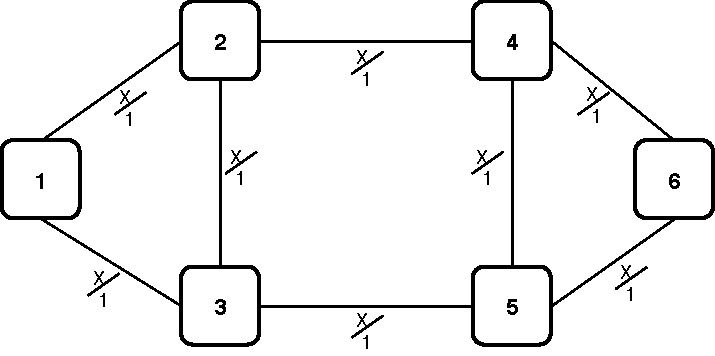
\includegraphics[width=11cm]{sdf/ilp/opaque_survivability/figures/allowed_physical_topology}
\caption{Allowed Physical Topology.}
\label{allowed_physical_medium}
\end{figure}

\begin{figure}[h!]
\centering
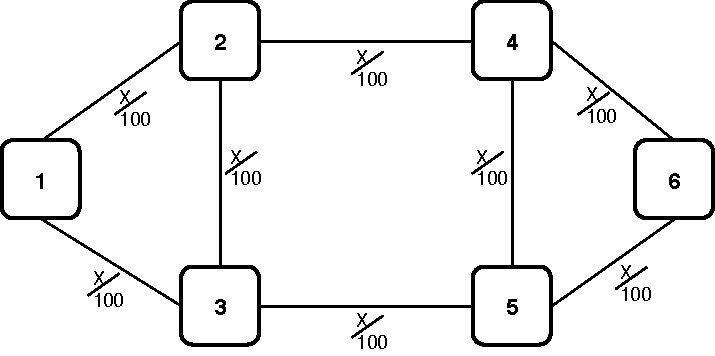
\includegraphics[width=12cm]{sdf/ilp/opaque_survivability/figures/allowed_optical_topology}
\caption{Allowed Optical Topology.}
\label{allowed_optical_medium}
\end{figure}

\begin{figure}[h!]
\centering
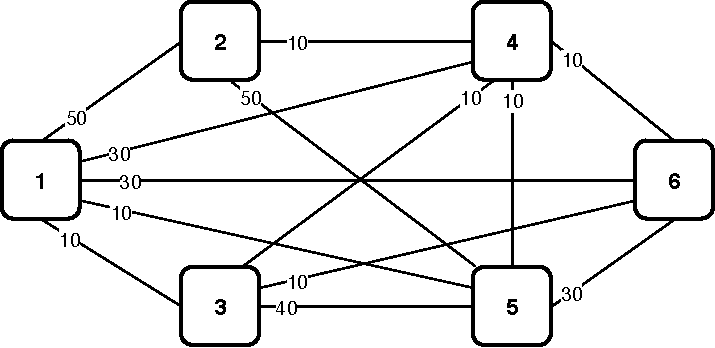
\includegraphics[width=12cm]{sdf/ilp/opaque_survivability/figures/logical_topology_ODU0_medium}
\caption{Logical Topology of ODU0.}
\label{logical_ODU0_medium}
\end{figure}

\begin{figure}[h!]
\centering
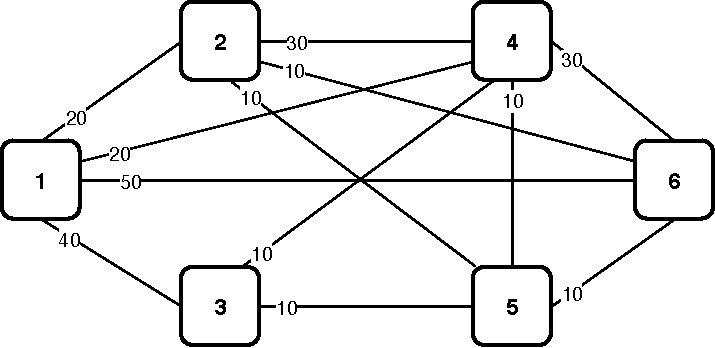
\includegraphics[width=12cm]{sdf/ilp/opaque_survivability/figures/logical_topology_ODU1_medium}
\caption{Logical Topology of ODU1.}
\label{logical_ODU1_medium}
\end{figure}

\begin{figure}[h!]
\centering
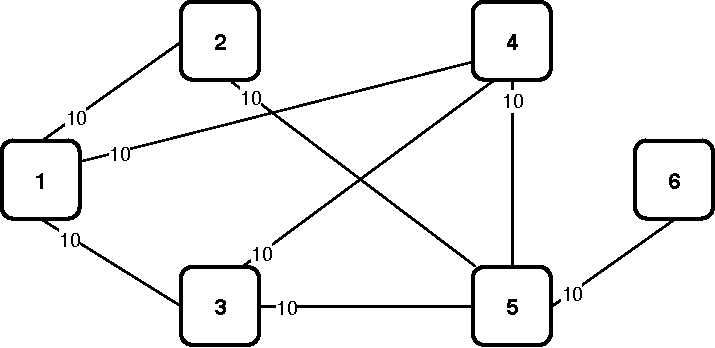
\includegraphics[width=12cm]{sdf/ilp/opaque_survivability/figures/logical_topology_ODU2_medium}
\caption{Logical Topology of ODU2.}
\label{logical_ODU2_medium}
\end{figure}

\begin{figure}[h!]
\centering
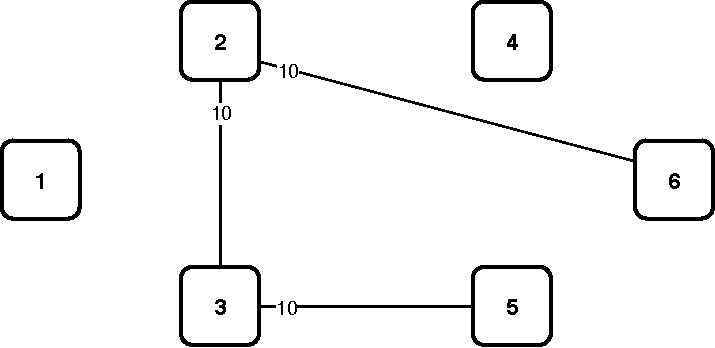
\includegraphics[width=12cm]{sdf/ilp/opaque_survivability/figures/logical_topology_ODU3_medium}
\caption{Logical Topology of ODU3.}
\label{logical_ODU3_medium}
\end{figure}

\begin{figure}[h!]
\centering
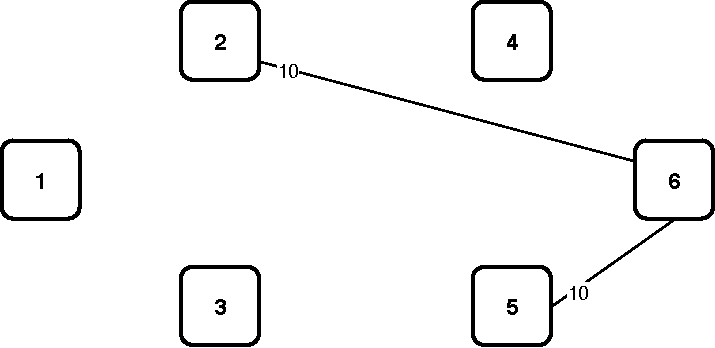
\includegraphics[width=12cm]{sdf/ilp/opaque_survivability/figures/logical_topology_ODU4_medium}
\caption{Logical Topology of ODU4.}
\label{logical_ODU4_medium}
\end{figure}

\begin{figure}[h!]
\centering
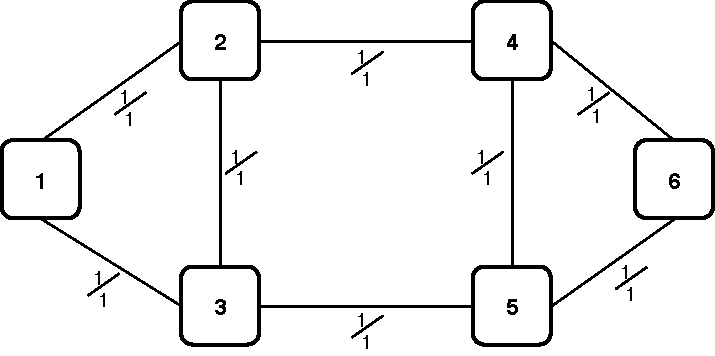
\includegraphics[width=12cm]{sdf/ilp/opaque_survivability/figures/physical_topology}
\caption{Physical Topology.}
\label{physical_medium}
\end{figure}

\begin{figure}[h!]
\centering
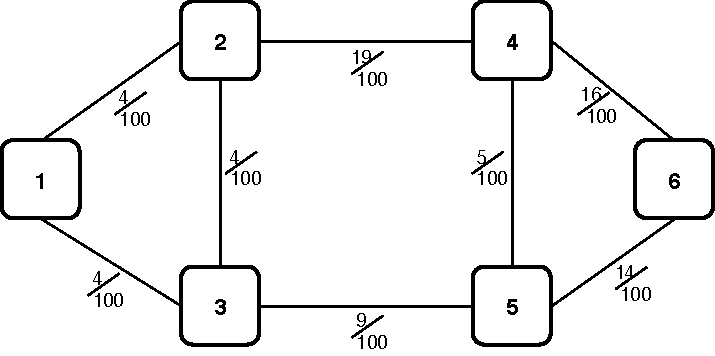
\includegraphics[width=12cm]{sdf/ilp/opaque_survivability/figures/optical_topology_medium}
\caption{Optical Topology.}
\label{optical_medium}
\end{figure}


In table \ref{link_opaque_surv_ref_medium} we can see the number of optical channels and the number of amplifiers for each link calculated through MatLab.

\begin{table}[h!]
\centering
\begin{tabular}{|| c | c | c ||}
 \hline
 \multicolumn{3}{|| c ||}{Information regarding links} \\
 \hline
 \hline
 Bidirectional Link & Optical Channels & Amplifiers\\
 \hline
 Node 1 <-> Node 2 & 4 & 4 \\
 Node 1 <-> Node 3 & 4 & 6 \\
 Node 2 <-> Node 3 & 4 & 0 \\
 Node 2 <-> Node 4 & 19 & 6 \\
 Node 3 <-> Node 5 & 9 & 8 \\
 Node 4 <-> Node 5 & 5 & 1 \\
 Node 4 <-> Node 6 & 16 & 7 \\
 Node 5 <-> Node 6 & 14 & 3 \\
 \hline
\end{tabular}
\caption{Table with information regarding links}
\label{link_opaque_surv_ref_medium}
\end{table}

In table \ref{node_opaque_surv_ref_medium} we can see the number of connections that each node has, the number of line ports and the number of tributary ports for each node.

\begin{table}[h!]
\centering
\begin{tabular}{|| c | c | c | c ||}
 \hline
 \multicolumn{4}{|| c ||}{Information regarding nodes} \\
 \hline
 \hline
 Node & Resulting Nodal Degree & Line Ports & Tributary Ports\\
 \hline
 1 & 2 & 8 & 290 \\
 2 & 3 & 27 & 230 \\
 3 & 3 & 17 & 180 \\
 4 & 3 & 40 & 200 \\
 5 & 3 & 28 & 240 \\
 6 & 2 & 30 & 220 \\
\hline
\end{tabular}
\caption{Table with information regarding nodes}
\label{node_opaque_surv_ref_medium}
\end{table}

In each table with detailed information we can see how many ports are connected to a given node and its bit rate (in relation to the line ports) and how many ports are assigned to each different bit rate (in relation to the tributary ports).

\begin{table}[h!]
\centering
\begin{tabular}{|| c | c | c ||}
 \hline
 \multicolumn{3}{|| c ||}{Detailed description of Node 1} \\
 \hline
 \hline
\multirow{2}{*}{8 line ports} & 4 connect to Node 2 & \multirow{2}{*}{100 Gbtis/s} \\
 & 4 connect to Node 3 & \\ \hline
\multirow{3}{*}{290 tributary ports} & 130 & ODU0 \\
 & 130 & ODU1 \\
 & 30 & ODU2 \\
\hline
\end{tabular}
\caption{Table with detailed description of node 1}
\end{table}

\newpage
\begin{table}[h!]
\centering
\begin{tabular}{|| c | c | c ||}
 \hline
 \multicolumn{3}{|| c ||}{Detailed description of Node 2} \\
 \hline
 \hline
 \multirow{3}{*}{27 line ports} & 4 connect to Node 1 & \multirow{3}{*}{100 Gbtis/s}\\
 & 4 connect to Node 3 & \\
 & 19 connect to Node 4 & \\ \hline
\multirow{5}{*}{230 tributary ports} & 110 & ODU0 \\
 & 70 & ODU1 \\
 & 20 & ODU2 \\
 & 20 & ODU3 \\
 & 10 & ODU4 \\
\hline
\end{tabular}
\caption{Table with detailed description of node 2}
\end{table}

\vspace{17pt}
\begin{table}[h!]
\centering
\begin{tabular}{|| c | c | c ||}
 \hline
 \multicolumn{3}{|| c ||}{Detailed description of Node 3} \\
 \hline
 \hline
 \multirow{3}{*}{17 line ports} & 4 connect to Node 1 & \multirow{3}{*}{100 Gbtis/s}\\
 & 4 connect to Node 2 & \\
 & 9 connect to Node 5 & \\ \hline
\multirow{4}{*}{180 tributary ports} & 70 & ODU0 \\
 & 60 & ODU1\\
 & 30 & ODU2\\
 & 20 & ODU3\\
\hline
\end{tabular}
\caption{Table with detailed description of node 3}
\end{table}

\vspace{17pt}
\begin{table}[h!]
\centering
\begin{tabular}{|| c | c | c ||}
 \hline
 \multicolumn{3}{|| c ||}{Detailed description of Node 4} \\
 \hline
 \hline
\multirow{3}{*}{40 line ports} & 19 connect to Node 2 & \multirow{3}{*}{100 Gbtis/s}\\
 & 5 connect to Node 5 & \\
 & 16 connect to Node 6 & \\ \hline
\multirow{3}{*}{200 tributary ports} & 70 & ODU0 \\
 & 100 & ODU1 \\
 & 30 & ODU2 \\
\hline
\end{tabular}
\caption{Table with detailed description of node 4}
\end{table}

\newpage
\begin{table}[h!]
\centering
\begin{tabular}{|| c | c | c ||}
 \hline
 \multicolumn{3}{|| c ||}{Detailed description of Node 5} \\
 \hline
 \hline
 \multirow{3}{*}{28 line ports} & 9 connect to Node 3 & \multirow{3}{*}{100 Gbtis/s} \\
 & 5 connect to Node 4 & \\
 & 14 connect to Node 6 & \\ \hline
\multirow{5}{*}{240 tributary ports} & 140 & ODU0 \\
 & 40 & ODU1 \\
 & 40 & ODU2 \\
 & 10 & ODU3 \\
 & 10 & ODU4 \\
\hline
\end{tabular}
\caption{Table with detailed description of node 5}
\end{table}

\begin{table}[h!]
\centering
\begin{tabular}{|| c | c | c ||}
 \hline
 \multicolumn{3}{|| c ||}{Detailed description of Node 6} \\
 \hline
 \hline
 \multirow{2}{*}{30 line ports} & 16 connect to Node 4 & \multirow{2}{*}{100 Gbtis/s} \\
 & 14 connect to Node 5 & \\ \hline
\multirow{5}{*}{220 tributary ports} & 80 & ODU0 \\
 & 100 & ODU1 \\
 & 10 & ODU2 \\
 & 10 & ODU3 \\
 & 20 & ODU4 \\
\hline
\end{tabular}
\caption{Table with detailed description of node 6}
\end{table}

Now through the table \ref{scriptopaque_surv_ref_medium} we can see the result of CAPEX obtained with this ILP model.

\begin{table}[h!]
\centering
\begin{tabular}{|| c | c | c | c | c | c | c ||}
 \hline
 \multicolumn{7}{|| c ||}{CAPEX of the Network} \\
 \hline
 \hline
 \multicolumn{3}{|| c |}{ } & Quantity & Unit Price & Cost & Total \\
 \hline
 \multirow{3}{*}{Link Cost} & \multicolumn{2}{ c |}{OLTs} & 16 & 15 000 \euro & 240 000 \euro & \multirow{3}{*}{75 520 000 \euro} \\ \cline{2-6}
 & \multicolumn{2}{ c |}{100 Gb/s Transceivers} & 150 & 5 000 \euro/Gb/s & 75 000 000 \euro & \\ \cline{2-6}
 & \multicolumn{2}{ c |}{Amplifiers} & 70 & 4 000 \euro & 280 000 \euro & \\
 \hline
 \multirow{9}{*}{Node Cost} & \multirow{7}{*}{Electrical} & EXCs & 6 & 10 000 \euro & 60 000 \euro & \multirow{9}{*}{15 085 900 \euro} \\ \cline{3-6}
 & & ODU0 Ports & 600 & 8 \euro/Gb/s & 6 000 \euro & \\ \cline{3-6}
 & & ODU1 Ports & 500 & 6 \euro/Gb/s & 7 500 \euro & \\ \cline{3-6}
 & & ODU2 Ports & 160 & 3 \euro/Gb/s & 4 800 \euro & \\ \cline{3-6}
 & & ODU3 Ports & 60 & 1.5 \euro/Gb/s & 3 600 \euro & \\ \cline{3-6}
 & & ODU4 Ports & 40 & 1 \euro/Gb/s & 4 000 \euro & \\ \cline{3-6}
 & & Line Ports & 150 & 1 000 \euro/Gb/s & 15 000 000 \euro & \\ \cline{2-6}
 & \multirow{2}{*}{Optical} & OXCs & 0 & 20 000 \euro & 0 \euro & \\ \cline{3-6}
 & & Ports & 0 & 2 500 \euro/porto & 0 \euro & \\
 \hline
 \multicolumn{6}{|| c |}{Total Network Cost} & 90 605 900 \euro \\
\hline
\end{tabular}
\caption{Table with detailed description of CAPEX}
\label{scriptopaque_surv_ref_medium}
\end{table}

\newpage
Through the formulas mentioned below we can see how all the values of the quantity column were calculated.

\begin{table}[h!]
\centering
\begin{tabular}{|| c | c ||}
 \hline
 OLTs: & \(\displaystyle 2 \sum_{i=1}^{N}\sum_{j=i+1}^{N} L_{ij} \) \\ \hline
 Transceivers: & \(\displaystyle 2 \sum_{i=1}^{N}\sum_{j=i+1}^{N} W_{ij} \) \\ \hline
 Amplifiers: & \(\displaystyle \sum_{i=1}^{N}\sum_{j=i+1}^{N} N^R_{ij} L_{ij} \) \\ \hline
 EXCs: & \(\displaystyle \sum_n^N N_{EXC,n} \) \\ \hline
 ODU0: & \(\displaystyle \sum_{o=1}^{N}\sum_{d=1}^{N} D_{od,0} \) \\ \hline
 ODU1: & \(\displaystyle \sum_{o=1}^{N}\sum_{d=1}^{N} D_{od,1} \) \\ \hline
 ODU2: & \(\displaystyle \sum_{o=1}^{N}\sum_{d=1}^{N} D_{od,2} \)\\ \hline
 ODU3: & \(\displaystyle \sum_{o=1}^{N}\sum_{d=1}^{N} D_{od,3} \) \\ \hline
 ODU4: & \(\displaystyle \sum_{o=1}^{N}\sum_{d=1}^{N} D_{od,4} \) \\ \hline
 Line: & \(\displaystyle \sum_{i=1}^{N}\sum_{j=1}^{N} W_{ij} \) \\ \hline
 OXCs: & As mentioned initially this result is always zero. \\ \hline
 Ports: & Does not exist for this case then it is equal to zero. \\
 \hline
 \end{tabular}
\caption{Table with description of calculation}
\label{formulas_opaque_surv_ref_medium}
\end{table}

\vspace{13pt}
It should be mentioned again that for all these final results it was necessary to take into account some restrictions, which are:
\begin{itemize}
  \item The solution is possible or impossible (we discard the case in which there is blocking).
  \item Each link only supports one transmission system.
  \item All demands have to follow the same path.
\end{itemize}

\newpage
Finally let's focus on the routing information. These paths are bidirectional so the path from one node to another is the same path in the opposite direction. In table \ref{path_opaque_surv_ref_medium} we can see all the routing obtained for all nodes.\\

\begin{table}[h!]
\centering
\begin{tabular}{|| c | c | c ||}
 \hline
 \multicolumn{3}{|| c ||}{Routing} \\
 \hline
 \hline
 o & d & Links \\
 \hline
 1 & 2 & \{(1,2)\} \\ \hline
 1 & 3 & \{(1,3)\} \\ \hline
 1 & 4 & \{(1,2),(2,4)\}\\ \hline
 1 & 5 & \{(1,3),(3,5)\}\\ \hline
 1 & 6 & \{(1,3),(3,5),(5,6)\}\\ \hline
 2 & 3 & \{(2,3)\}\\ \hline
 2 & 4 & \{(2,4)\}\\ \hline
 2 & 5 & \{(2,4),(4,5)\}\\ \hline
 2 & 6 & \{(2,4),(4,6)\}\\ \hline
 3 & 4 & \{(3,5),(5,4)\}\\ \hline
 3 & 5 & \{(3,5)\}\\ \hline
 3 & 6 & \{(3,5),(5,6)\}\\ \hline
 4 & 5 & \{(4,5)\}\\ \hline
 4 & 6 & \{(4,6)\}\\ \hline
 5 & 6 & \{(5,6)\}\\
 \hline
\end{tabular}
\caption{Table with description of routing}
\label{path_opaque_surv_ref_medium}
\end{table}


\vspace{20pt}
\textbf{High Traffic Scenario:}\\

In this scenario we have to take into account the traffic calculated in \ref{high_traffic_scenario}. In a first phase we will show the various exiting topologies of the network. The first are the allowed topologies, physical and optical topology, the second are the logical topology for all ODUs and finally the resulting physical and optical topology.\\
\newpage
\begin{figure}[h!]
\centering
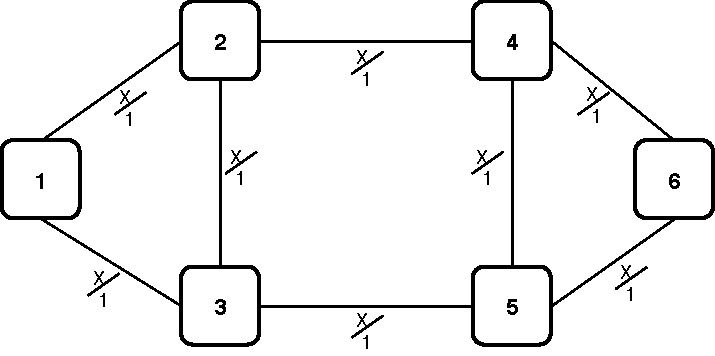
\includegraphics[width=11cm]{sdf/ilp/opaque_survivability/figures/allowed_physical_topology}
\caption{Allowed Physical Topology.}
\label{allowed_physical_high}
\end{figure}

\begin{figure}[h!]
\centering
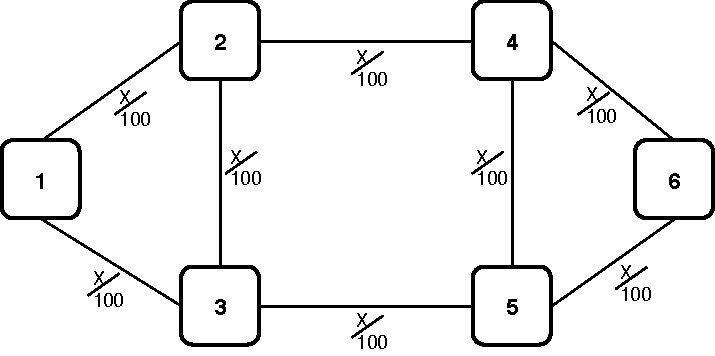
\includegraphics[width=12cm]{sdf/ilp/opaque_survivability/figures/allowed_optical_topology}
\caption{Allowed Optical Topology.}
\label{allowed_optical_high}
\end{figure}

\begin{figure}[h!]
\centering
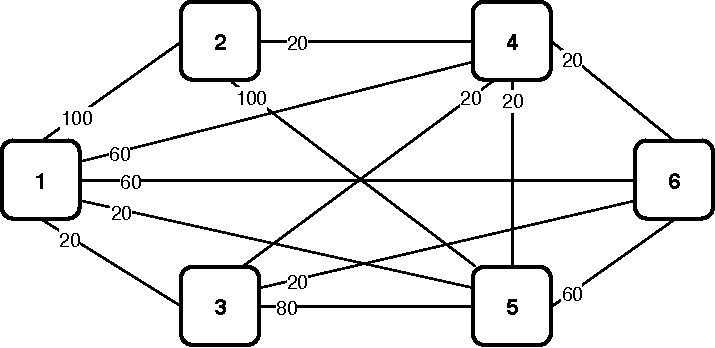
\includegraphics[width=12cm]{sdf/ilp/opaque_survivability/figures/logical_topology_ODU0_high}
\caption{Logical Topology of ODU0.}
\label{logical_ODU0_high}
\end{figure}

\begin{figure}[h!]
\centering
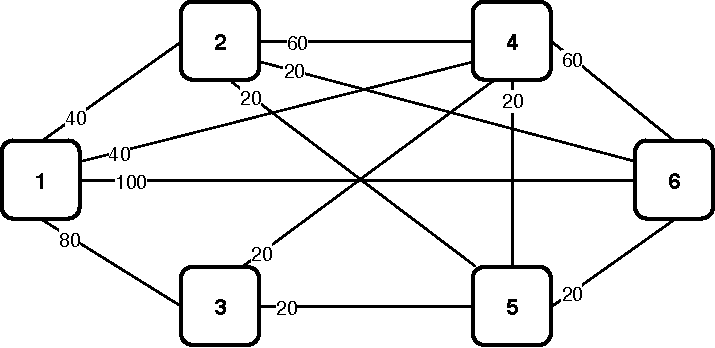
\includegraphics[width=12cm]{sdf/ilp/opaque_survivability/figures/logical_topology_ODU1_high}
\caption{Logical Topology of ODU1.}
\label{logical_ODU1_high}
\end{figure}

\begin{figure}[h!]
\centering
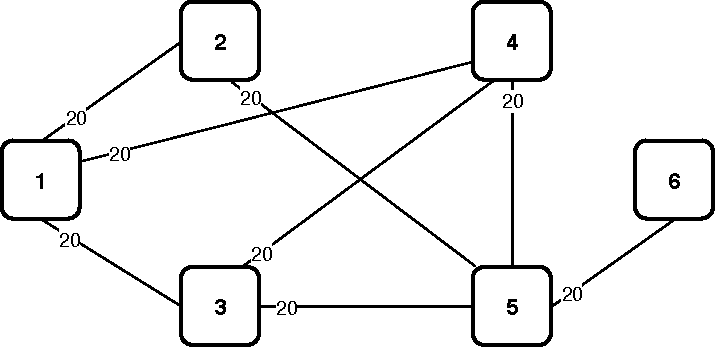
\includegraphics[width=12cm]{sdf/ilp/opaque_survivability/figures/logical_topology_ODU2_high}
\caption{Logical Topology of ODU2.}
\label{logical_ODU2_high}
\end{figure}

\begin{figure}[h!]
\centering
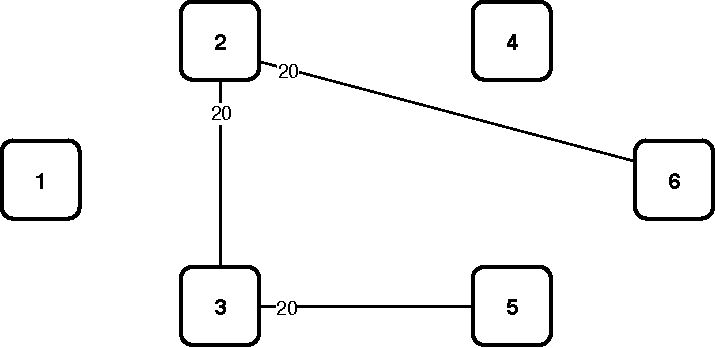
\includegraphics[width=12cm]{sdf/ilp/opaque_survivability/figures/logical_topology_ODU3_high}
\caption{Logical Topology of ODU3.}
\label{logical_ODU3_high}
\end{figure}

\begin{figure}[h!]
\centering
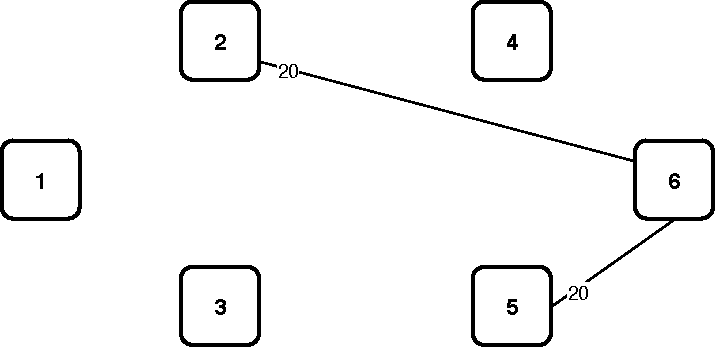
\includegraphics[width=12cm]{sdf/ilp/opaque_survivability/figures/logical_topology_ODU4_high}
\caption{Logical Topology of ODU4.}
\label{logical_ODU4_high}
\end{figure}

\begin{figure}[h!]
\centering
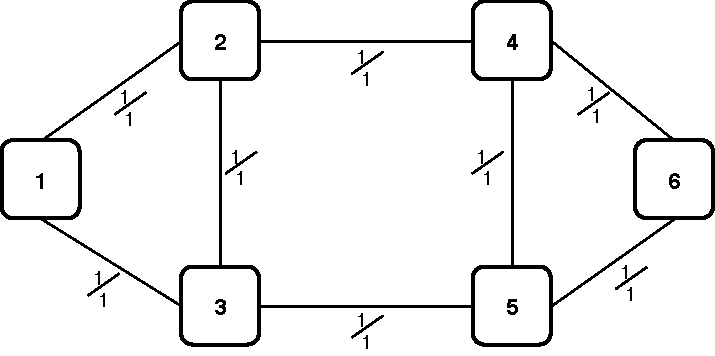
\includegraphics[width=12cm]{sdf/ilp/opaque_survivability/figures/physical_topology}
\caption{Physical Topology.}
\label{physical_high}
\end{figure}

\begin{figure}[h!]
\centering
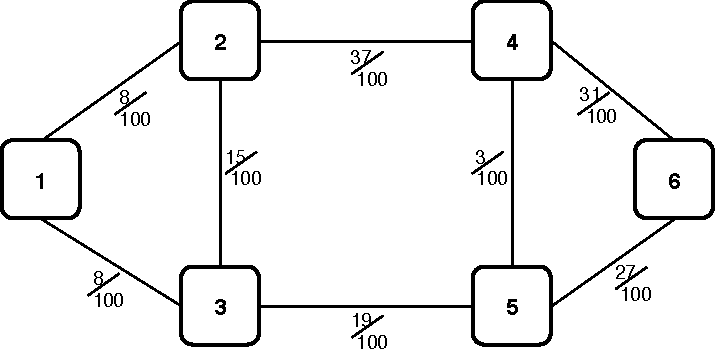
\includegraphics[width=12cm]{sdf/ilp/opaque_survivability/figures/optical_topology_high}
\caption{Optical Topology.}
\label{optical_high}
\end{figure}

\newpage
In table \ref{link_opaque_surv_ref_high} we can see the number of optical channels and the number of amplifiers for each link calculated through MatLab.

\begin{table}[h!]
\centering
\begin{tabular}{|| c | c | c ||}
 \hline
 \multicolumn{3}{|| c ||}{Information regarding links} \\
 \hline
 \hline
 Bidirectional Link & Optical Channels & Amplifiers\\
 \hline
 Node 1 <-> Node 2 & 8 & 4 \\
 Node 1 <-> Node 3 & 8 & 6 \\
 Node 2 <-> Node 3 & 15 & 0 \\
 Node 2 <-> Node 4 & 37 & 6 \\
 Node 3 <-> Node 5 & 19 & 8 \\
 Node 4 <-> Node 5 & 3 & 1 \\
 Node 4 <-> Node 6 & 31 & 7 \\
 Node 5 <-> Node 6 & 27 & 3 \\
 \hline
\end{tabular}
\caption{Table with information regarding links}
\label{link_opaque_surv_ref_high}
\end{table}

In table \ref{node_opaque_surv_ref_high} we can see the number of connections that each node has, the number of line ports and the number of tributary ports for each node.

\begin{table}[h!]
\centering
\begin{tabular}{|| c | c | c | c ||}
 \hline
 \multicolumn{4}{|| c ||}{Information regarding nodes} \\
 \hline
 \hline
 Node & Resulting Nodal Degree & Line Ports & Tributary Ports\\
 \hline
 1 & 2 & 16 & 580 \\
 2 & 3 & 60 & 460 \\
 3 & 3 & 42 & 360 \\
 4 & 3 & 71 & 400 \\
 5 & 3 & 49 & 480 \\
 6 & 2 & 58 & 440 \\
\hline
\end{tabular}
\caption{Table with information regarding nodes}
\label{node_opaque_surv_ref_high}
\end{table}

In each table mentioned below with detailed information we can see how many ports are connected to a given node and its bit rate (in relation to the line ports) and how many ports are assigned to each different bit rate (in relation to the tributary ports).

\begin{table}[h!]
\centering
\begin{tabular}{|| c | c | c ||}
 \hline
 \multicolumn{3}{|| c ||}{Detailed description of Node 1} \\
 \hline
 \hline
\multirow{2}{*}{16 line ports} & 8 connect to Node 2 & \multirow{2}{*}{100 Gbtis/s} \\
 & 8 connect to Node 3 & \\ \hline
\multirow{3}{*}{580 tributary ports} & 260 & ODU0 \\
 & 260 & ODU1 \\
 & 60 & ODU2 \\
\hline
\end{tabular}
\caption{Table with detailed description of node 1}
\end{table}

\newpage
\begin{table}[h!]
\centering
\begin{tabular}{|| c | c | c ||}
 \hline
 \multicolumn{3}{|| c ||}{Detailed description of Node 2} \\
 \hline
 \hline
 \multirow{3}{*}{60 line ports} & 8 connect to Node 1 & \multirow{3}{*}{100 Gbtis/s}\\
 & 15 connect to Node 3 & \\
 & 37 connect to Node 4 & \\ \hline
\multirow{5}{*}{460 tributary ports} & 220 & ODU0 \\
 & 140 & ODU1 \\
 & 40 & ODU2 \\
 & 40 & ODU3 \\
 & 20 & ODU4 \\
\hline
\end{tabular}
\caption{Table with detailed description of node 2}
\end{table}

\vspace{17pt}
\begin{table}[h!]
\centering
\begin{tabular}{|| c | c | c ||}
 \hline
 \multicolumn{3}{|| c ||}{Detailed description of Node 3} \\
 \hline
 \hline
 \multirow{3}{*}{42 line ports} & 8 connect to Node 1 & \multirow{3}{*}{100 Gbtis/s}\\
 & 15 connect to Node 2 & \\
 & 19 connect to Node 5 & \\ \hline
\multirow{4}{*}{360 tributary ports} & 140 & ODU0 \\
 & 120 & ODU1\\
 & 60 & ODU2\\
 & 40 & ODU3\\
\hline
\end{tabular}
\caption{Table with detailed description of node 3}
\end{table}

\vspace{17pt}
\begin{table}[h!]
\centering
\begin{tabular}{|| c | c | c ||}
 \hline
 \multicolumn{3}{|| c ||}{Detailed description of Node 4} \\
 \hline
 \hline
\multirow{3}{*}{71 line ports} & 37 connect to Node 2 & \multirow{3}{*}{100 Gbtis/s}\\
 & 3 connect to Node 5 & \\
 & 31 connect to Node 6 & \\ \hline
\multirow{3}{*}{400 tributary ports} & 140 & ODU0 \\
 & 200 & ODU1 \\
 & 60 & ODU2 \\
\hline
\end{tabular}
\caption{Table with detailed description of node 4}
\end{table}

\newpage
\begin{table}[h!]
\centering
\begin{tabular}{|| c | c | c ||}
 \hline
 \multicolumn{3}{|| c ||}{Detailed description of Node 5} \\
 \hline
 \hline
 \multirow{3}{*}{49 line ports} & 19 connect to Node 3 & \multirow{3}{*}{100 Gbtis/s} \\
 & 3 connect to Node 4 & \\
 & 27 connect to Node 6 & \\ \hline
\multirow{5}{*}{480 tributary ports} & 280 & ODU0 \\
 & 80 & ODU1 \\
 & 80 & ODU2 \\
 & 20 & ODU3 \\
 & 20 & ODU4 \\
\hline
\end{tabular}
\caption{Table with detailed description of node 5}
\end{table}

\begin{table}[h!]
\centering
\begin{tabular}{|| c | c | c ||}
 \hline
 \multicolumn{3}{|| c ||}{Detailed description of Node 6} \\
 \hline
 \hline
 \multirow{2}{*}{58 line ports} & 31 connect to Node 4 & \multirow{2}{*}{100 Gbtis/s} \\
 & 27 connect to Node 5 & \\ \hline
\multirow{5}{*}{440 tributary ports} & 160 & ODU0 \\
 & 200 & ODU1 \\
 & 20 & ODU2 \\
 & 20 & ODU3 \\
 & 40 & ODU4 \\
\hline
\end{tabular}
\caption{Table with detailed description of node 6}
\end{table}

Now through the table \ref{scriptopaque_surv_ref_high} we can see the result of CAPEX obtained with this ILP model.

\begin{table}[h!]
\centering
\begin{tabular}{|| c | c | c | c | c | c | c ||}
 \hline
 \multicolumn{7}{|| c ||}{CAPEX of the Network} \\
 \hline
 \hline
 \multicolumn{3}{|| c |}{ } & Quantity & Unit Price & Cost & Total \\
 \hline
 \multirow{3}{*}{Link Cost} & \multicolumn{2}{ c |}{OLTs} & 16 & 15 000 \euro & 240 000 \euro & \multirow{3}{*}{148 520 000 \euro} \\ \cline{2-6}
 & \multicolumn{2}{ c |}{100 Gb/s Transceivers} & 296 & 5 000 \euro/Gb/s & 148 000 000 \euro & \\ \cline{2-6}
 & \multicolumn{2}{ c |}{Amplifiers} & 70 & 4 000 \euro & 280 000 \euro & \\
 \hline
 \multirow{9}{*}{Node Cost} & \multirow{7}{*}{Electrical} & EXCs & 6 & 10 000 \euro & 60 000 \euro & \multirow{9}{*}{29 711 800 \euro} \\ \cline{3-6}
 & & ODU0 Ports & 1 200 & 8 \euro/Gb/s & 12 000 \euro & \\ \cline{3-6}
 & & ODU1 Ports & 1 000 & 6 \euro/Gb/s & 15 000 \euro & \\ \cline{3-6}
 & & ODU2 Ports & 320 & 3 \euro/Gb/s & 9 600 \euro & \\ \cline{3-6}
 & & ODU3 Ports & 120 & 1.5 \euro/Gb/s & 7 200 \euro & \\ \cline{3-6}
 & & ODU4 Ports & 80 & 1 \euro/Gb/s & 8 000 \euro & \\ \cline{3-6}
 & & Line Ports & 296 & 1 000 \euro/Gb/s & 29 600 000 \euro & \\ \cline{2-6}
 & \multirow{2}{*}{Optical} & OXCs & 0 & 20 000 \euro & 0 \euro & \\ \cline{3-6}
 & & Ports & 0 & 2 500 \euro/porto & 0 \euro & \\
 \hline
 \multicolumn{6}{|| c |}{Total Network Cost} & 178 231 800 \euro \\
\hline
\end{tabular}
\caption{Table with detailed description of CAPEX}
\label{scriptopaque_surv_ref_high}
\end{table}

\newpage
Through the formulas mentioned below we can see how all the values of the quantity column were calculated.

\begin{table}[h!]
\centering
\begin{tabular}{|| c | c ||}
 \hline
 OLTs: & \(\displaystyle 2 \sum_{i=1}^{N}\sum_{j=i+1}^{N} L_{ij} \) \\ \hline
 Transceivers: & \(\displaystyle 2 \sum_{i=1}^{N}\sum_{j=i+1}^{N} W_{ij} \) \\ \hline
 Amplifiers: & \(\displaystyle \sum_{i=1}^{N}\sum_{j=i+1}^{N} N^R_{ij} L_{ij} \) \\ \hline
 EXCs: & \(\displaystyle \sum_n^N N_{EXC,n} \) \\ \hline
 ODU0: & \(\displaystyle \sum_{o=1}^{N}\sum_{d=1}^{N} D_{od,0} \) \\ \hline
 ODU1: & \(\displaystyle \sum_{o=1}^{N}\sum_{d=1}^{N} D_{od,1} \) \\ \hline
 ODU2: & \(\displaystyle \sum_{o=1}^{N}\sum_{d=1}^{N} D_{od,2} \)\\ \hline
 ODU3: & \(\displaystyle \sum_{o=1}^{N}\sum_{d=1}^{N} D_{od,3} \) \\ \hline
 ODU4: & \(\displaystyle \sum_{o=1}^{N}\sum_{d=1}^{N} D_{od,4} \) \\ \hline
 Line: & \(\displaystyle \sum_{i=1}^{N}\sum_{j=1}^{N} W_{ij} \) \\ \hline
 OXCs: & As mentioned initially this result is always zero. \\ \hline
 Ports: & Does not exist for this case then it is equal to zero. \\
 \hline
 \end{tabular}
\caption{Table with description of calculation}
\label{formulas_opaque_surv_ref_high}
\end{table}

\vspace{13pt}
It should be mentioned again that for all these final results it was necessary to take into account some restrictions, which are:
\begin{itemize}
  \item The solution is possible or impossible (we discard the case in which there is blocking).
  \item Each link only supports one transmission system.
  \item All demands have to follow the same path.
\end{itemize}

\newpage
Finally let's focus on the routing information. These paths are bidirectional so the path from one node to another is the same path in the opposite direction. In table \ref{path_opaque_surv_ref_high} we can see all the routing obtained for all nodes.\\

\begin{table}[h!]
\centering
\begin{tabular}{|| c | c | c ||}
 \hline
 \multicolumn{3}{|| c ||}{Routing} \\
 \hline
 \hline
 o & d & Links \\
 \hline
 1 & 2 & \{(1,2)\} \\ \hline
 1 & 3 & \{(1,3)\} \\ \hline
 1 & 4 & \{(1,2),(2,4)\}\\ \hline
 1 & 5 & \{(1,3),(3,5)\}\\ \hline
 1 & 6 & \{(1,3),(3,5),(5,6)\}\\ \hline
 2 & 3 & \{(2,3)\}\\ \hline
 2 & 4 & \{(2,4)\}\\ \hline
 2 & 5 & \{(2,3),(3,5)\}\\ \hline
 2 & 6 & \{(2,4),(4,6)\}\\ \hline
 3 & 4 & \{(3,2),(2,4)\}\\ \hline
 3 & 5 & \{(3,5)\}\\ \hline
 3 & 6 & \{(3,5),(5,6)\}\\ \hline
 4 & 5 & \{(4,5)\}\\ \hline
 4 & 6 & \{(4,6)\}\\ \hline
 5 & 6 & \{(5,6)\}\\
 \hline
\end{tabular}
\caption{Table with description of routing}
\label{path_opaque_surv_ref_high}
\end{table}

